%SDES_Project1
%Vikas Kurapti
%130010058
\documentclass[12pt, a4paper]{report}

\usepackage[affil-it]{authblk}
\usepackage{etoolbox}
\usepackage{lmodern}
\usepackage{titlesec}
\usepackage{float}
\usepackage{amsfonts}
\usepackage{graphicx}
\usepackage[pdfpagelabels]{hyperref}

\makeatletter
\patchcmd{\@maketitle}{\LARGE \@title}{\fontsize{20}{19.2}\selectfont\@title}{}{}
\makeatother

\renewcommand\Authfont{\fontsize{16}{14.4}\selectfont}
\renewcommand\Affilfont{\fontsize{12}{10.8}\itshape}

\title{\textbf{LC Tank with Resistance}}
\author{Vikas Kurapati}
\affil{Roll No. : 130010058}

\begin{document}
\maketitle
\newpage

\begin{abstract}
 The problem is to simulate the behaviour of a LC tank with a resistance applied across a voltage in series with given initial conditions of the charge in the capacitor and current in the inductor.
\end{abstract}

\begin{itemize}
\item Public git repo with open source code is available on \url{https://github.com/vikaskurapatibat/SDES_Project1}
\item Ipython 2.3.0 is used to run the IPython notebook. So the version 2.3.0 or higher is preferrable to run the notebook.
\item numpy version 1.8.2 is used. So numpy version 1.8.2 or higher is preffered to run the code.
\item matplotlib version 1.4.2 is used. So matplotlib version 1.4.2 or higher is preffered to run the code. 
\end{itemize}

\section*{Governing Equation for the problem}
The governing equation for this electrical problem is 
\begin{equation}
 \frac{d^2V_C}{dt^2} + \frac{R}{L}\frac{dV_C}{dt} + \frac{V_C}{LC} = \frac{V_S}{LC}
\end{equation}

where $V_C$ is the voltage across the capacitor varying with time, R is the resistance of the resistor, L is inductance of the inductor,C is the capacitance of the capacitor and $V_S$ is the voltage of the source voltage under the initial conditions of $V_C(0^+) = V_0$ the initial capacitor voltage and $\frac{dV_C}{dt}(0^+) = \frac{i_0}{C}$, where initial inductor current is $i_0$. \\

Solving this analytically for two cases of $\Delta = 0$ and $\Delta \ne 0$ where $\Delta = \frac{R^2}{L^2} - \frac{4}{LC}$ \\
\subsection*{$\Delta = 0$ :}
The solution when $\Delta = 0$ under the given initial conditions is:
\begin{equation}
 V_C(t) = V_S + e^\frac{-t}{2RC}(D_1t + D_2)
\end{equation}
where $D_1 = \frac{i_0}{C}e^\frac{1}{2RC} , D_2 = (V_0 - V)e^\frac{1}{2RC}$
\subsection*{$\Delta \ne 0$ :}
The solution when $\Delta \ne 0$ under the given initial conditions is:
\begin{equation}
 V_C(t) = V_0 + A_1e^{s_1t} + A_2e^{s_2t}
\end{equation}
where $s_1 = \frac{-R}{2L} + \frac{\sqrt{\Delta}}{2} , s_2 = \frac{-R}{2L} - \frac{\sqrt{\Delta}}{2}$ \\
$A_1 = \frac{\frac{i_0}{C} - (V_0 - V)s_2}{s_1 - s_2} , A_2 = \frac{\frac{i_0}{C} - (V_0 - V)s_1}{s_2 - s_1}$ \\
\\

The results were plotted showing the voltage accross a capacitor varying with time for three cases of damping.
\begin{figure}[H]
 \centering
 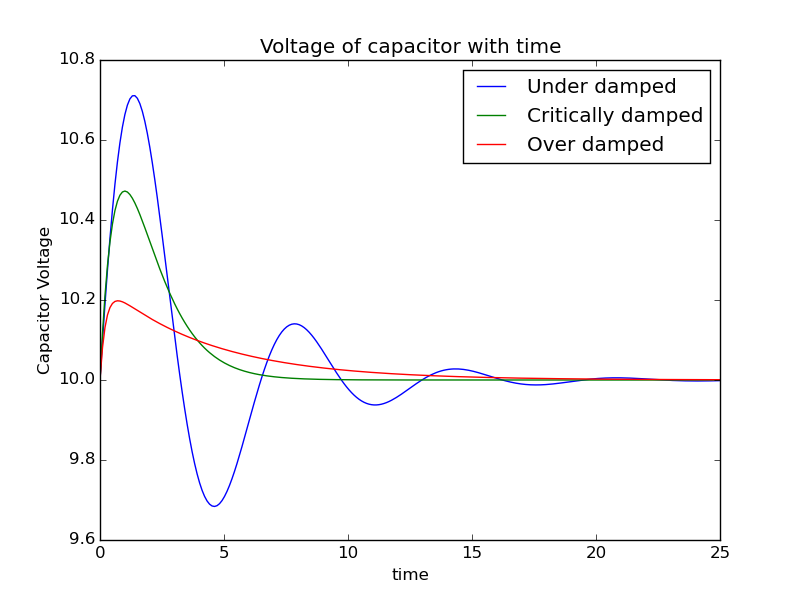
\includegraphics[width = \textwidth]{VC.png}
 \caption{$V_C$ vs time}
 \label{VC}
\end{figure}

\end{document}